\documentclass[twocolumn,amsmath,amssymb,aps]{revtex4}
\usepackage{graphicx}% Include figure files
\usepackage{dcolumn}% Align table columns on decimal point
\usepackage{bm}% bold math
\usepackage{color, subfigure}
\usepackage{csquotes}





\begin{document}
\title{Just How Complicated is the Complicated Dynamics in the Simple Logistic Map?}%
\author{Huan Q, Bui}\email{hqbui21@colby.edu}
\affiliation{Departent of Physics and Astronomy, Colby College.}
\date{\today}
\begin{abstract}
This paper focuses on the highly complex dynamics and various characteristics of the chaos which arise from the logistic map. In particular, the paper explores period-doubling cascades, the first Feigenbaum constant, and the connection to the Mandelbrot set.
\end{abstract}
\maketitle




\section{Introduction}
\textit{Chaos} in the technical sense refers to dynamical systems whose seemingly irregular and random behaviors are governed by deterministic law and are extremely sensitive to initial conditions. While it might seem counter-intuitive that determinism is one of the defining factors of chaos, there are in fact many such systems in nature. In hydrodynamics, the weather is a prime example: a collection of particles (the air) following deterministic rules as simple as momentum and energy conservation can manifest in behaviors so complex (the weather) that even the most powerful computers today cannot predict with certainty. The essence of chaos theory is perhaps best captured by Edward Lorenz -- one of the pioneers of the field:
\begin{displayquote}
``Chaos: When the present determines the future, but the approximate present does not approximately determine the future.''\cite{lorenz_quote}
\end{displayquote}
Chaos theory emerged in the 1960s following a number of discoveries in physics and mathematics, including Lorenz' famous paper titled ``Deterministic Nonperiodic Flow.'' In this paper, Lorenz explores a simplified  model for atmospheric convection consisting of three coupled ordinary differential equations. Now known as the \textit{Lorenz} \textit{system}, this model exhibits not only nonlinear and nonperiodic behavior, but also extreme sensitivity to perturbations in initial conditions characteristic of chaos.


Following Lorenz' discovery, Robert May extended the boundary of chaos theory through his work on the logistic difference equation (now known as the logistic map) in his 1976 paper ``{Simple mathematical models with very complicated dynamics}'' \cite{rmay76}. Starting with a very simple rule which resembles the regularity that emerges from the Lorenz system, Robert May showed that highly chaotic behaviors could in fact emerge. In Section II, we will explore these chaotic behaviors in more detail. We will also touch on some interesting and beautiful mathematical connections.





\section{The Logistic Map}

\subsection{Introduction}
The logistic map is a discrete-time iterative map. Unlike its continuous counter part, the logistic map recursively generates a sequence of numbers $\{x_n\}$ for every initial value $x_0$. The map takes the following functional form: 
\begin{equation*}
x_{k+1} = ax_k(1-  x_k)
\end{equation*}
where $a \in [0,4]$. The logistic map is related to the famous predator-prey model in ecology. As such, we can interpret the value $x_n \in [0,1]$ in the logistic map as the ratio of the existing population to the maximum possible population. The parameter $a$ is related to the growth rate of the population. When $a > 4$ or $a<0$, the sequence $\{x_n\}$ can have negative values or values that are greater than 1. As a result, the logistic map can only be interpreted in the ecological context when $a\in [0,4]$.

\subsection{Bifurcation Diagram}

There are many ways to study the dynamics of the model under different values of $a$. For example, Figures \ref{fig:cobweb} and \ref{fig:cobweb1} show cobweb plots, which among other variants of interactive plots allow the user to adjust various model parameters and initial conditions and readily see how the system reacts. Their objective is simple: to map out how the system evolves through the iterations. The cobweb method is a simple way to detect chaos. By looking at the behavior of the sequence $\{x_n\}$, one can determine whether it converges, diverges, or alternates between some set of values. 

\begin{figure}[!htb]
	\centering
	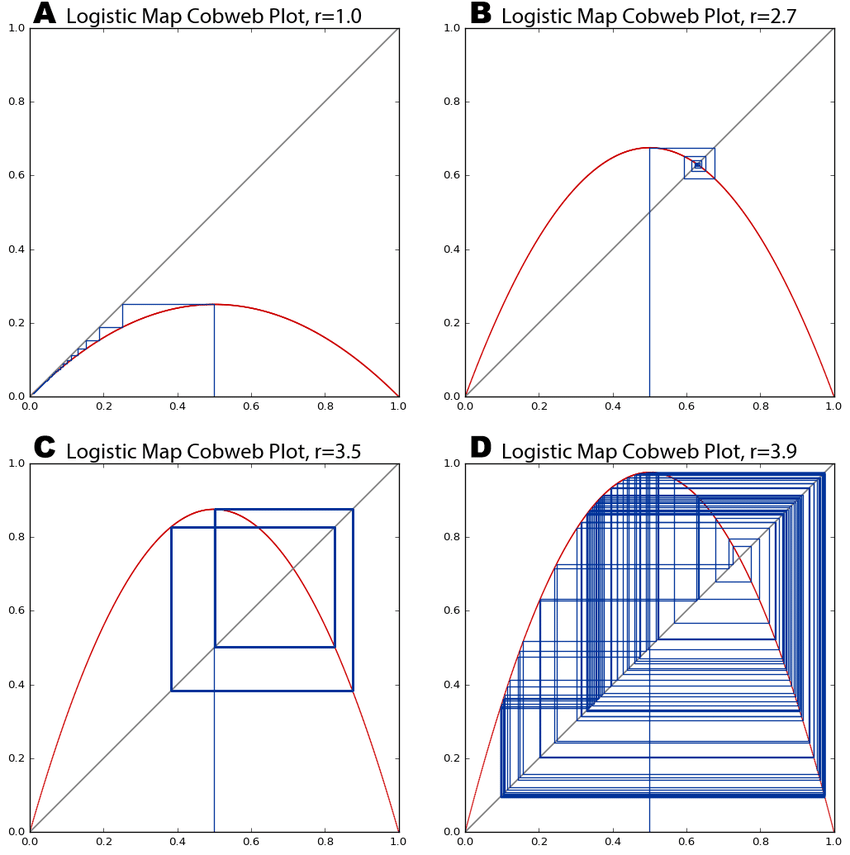
\includegraphics[scale=0.25]{cobweb}
	\caption{The system evolving from different values of $x_0$ and $a$. Courtesy of ``\textit{Methods and Measures for Analyzing Complex Street Networks and Urban Form} - Scientific Figure on ResearchGate.''}
	\label{fig:cobweb}
\end{figure}

\begin{figure}[!htb]
	\centering
	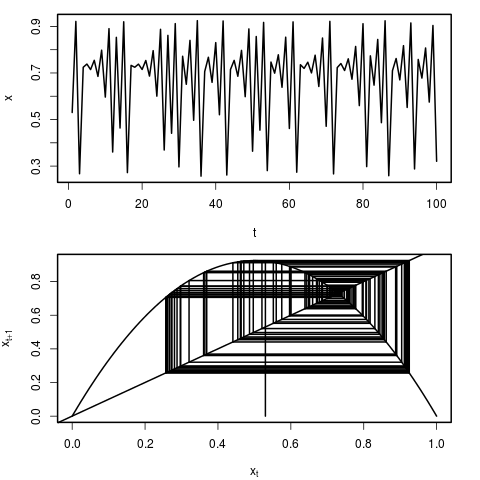
\includegraphics[scale=0.5]{cobweb_1}
	\caption{Top: $\{x_n\}$ plotted as a function of $n$. Bottom: how this evolution appears on the cobweb plot. Courtesy of ``The Bayesian Biologist''}
	\label{fig:cobweb1}
\end{figure}

A potential disadvantage of this method of analysis is, of course, information density. One can only display up to a few categorically different behaviors on one plot at a time before the plot loses clarity. To overcome this, we will consider and focus on for the rest of this paper the \textbf{bifurcation diagram}. Bifurcation diagrams are constructed by repeatedly plotting only the states of the system under various initial conditions after some iterations, for every value of $a$. The full bifurcation diagram for the logistic map is shown in Figure \ref{fig:logistic_2}.

\begin{figure}[!htb]
	\centering
	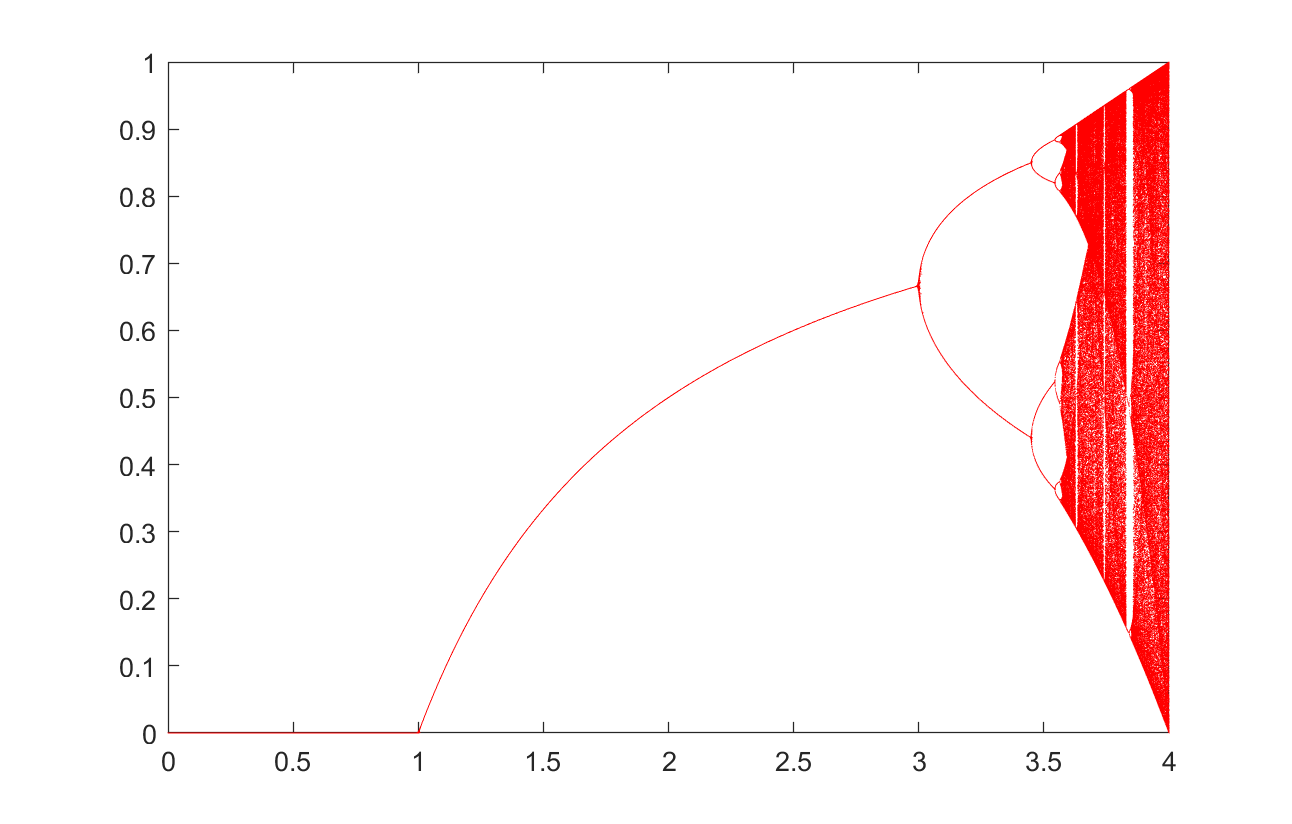
\includegraphics[scale=0.25]{logistic_2.png}
	\caption{Full bifurcation diagram, $a \in [0,4]$. The $x$-axis shows different values of $a$. The $y$-axis shows the final states of the system.}
	\label{fig:logistic_2}
\end{figure}




Bifurcation diagrams are a simple yet powerful tool to view chaos. Unlike in the cobweb method where one can be unsure of whether the system is purely chaotic or just highly periodic, bifurcation diagrams can show us with certainty what regime the system is in. This relies on the fact that chaos occurs exactly when the system becomes extremely sensitive to initial conditions. For example, let $a = 2$. It is clear from Figure \ref{fig:logistic_2} that all initial states $x_0\in [0,1]$ eventually converge to a single value $x_\infty \approx 0.5$; the system is non-chaotic. In contrast, when $a \approx 4$, the set of final states almost covers the entire interval $[0,1]$; the system is chaotic. 






\subsection{Period-Doubling Cascade of the ``First Order''}

In this subsection we begin to explore how the system behaves as $a$ ranges from $0$ to $4$ and observe the period-doubling cascade -- the most striking manifestation of complexity arising from the simple logistic map. To this end, we carefully follow the infinite-time behavior of the system as a function of $a$, using the bifurcation diagram introduced in the preceding section.

First, we find that for $a\in [0,1]$, the sequence $\{x_n\}$ converges to $0$ for any initial value $x_0\in [0,1]$. In ecological terms, we say that the population eventually vanishes. 

For $a\in [1,3]$, the sequence $\{x_n\}$ converges (see Figures \ref{fig:logistic_2} and \ref{fig:logistic_1}). As a result, we can show that $\{x_n\}$ approaches the fraction $(a-1)/a$:
\begin{eqnarray}
\lim_{n\to \infty} x_{n} &=& \lim_{n\to \infty} ax_{n-1}(1-x_{n-1}) \nonumber \\
&=& \lim_{n\to \infty} ax_{n}(1-x_{n}) \nonumber \\
\implies x_\infty &=& a x_\infty(1-x_\infty) \nonumber \\
x_\infty &=& \frac{a-1}{a} \nonumber,
\end{eqnarray}
which is also independent of $x_0$. Notice that we could derive this limit \textit{only because} we know in advance that the sequence converges to a single value. 

For $a > 3$, the convergence condition is no longer satisfied, and the derivation above becomes invalid. From this point on, we can only investigate the dynamics numerically. For $a$ between $3$ and $a_1 \approx 3.45$, we are one step closer to chaos. Within this interval, the system eventually oscillates between exactly 2 values which depend on $a$. See Figures \ref{fig:logistic_2} and \ref{fig:logistic_1} for better detail.

When $a\in [a_1,a_2]$ where $a_2 \approx 3.54$, the system eventually oscillates among 4 values, all of which again depend on $a$. We have observed the first \textbf{period-doubling}. Figure \ref{fig:logistic_3} shows only the top branch of the first bifurcation, which contains two of the four possible final values. The bottom branch contains the other two. 

In Figures \ref{fig:logistic_4} and \ref{fig:logistic_5}, we see that the system eventually oscillates between 8, 16, 32 values, and so on. By continually zooming into each bifurcation, we can find more period-doubling bifurcations of similar form. This self-similar, fractal-like structure is referred to as a \textbf{cascade} of period-doubling. 
\begin{figure}[!htb]
	\centering
	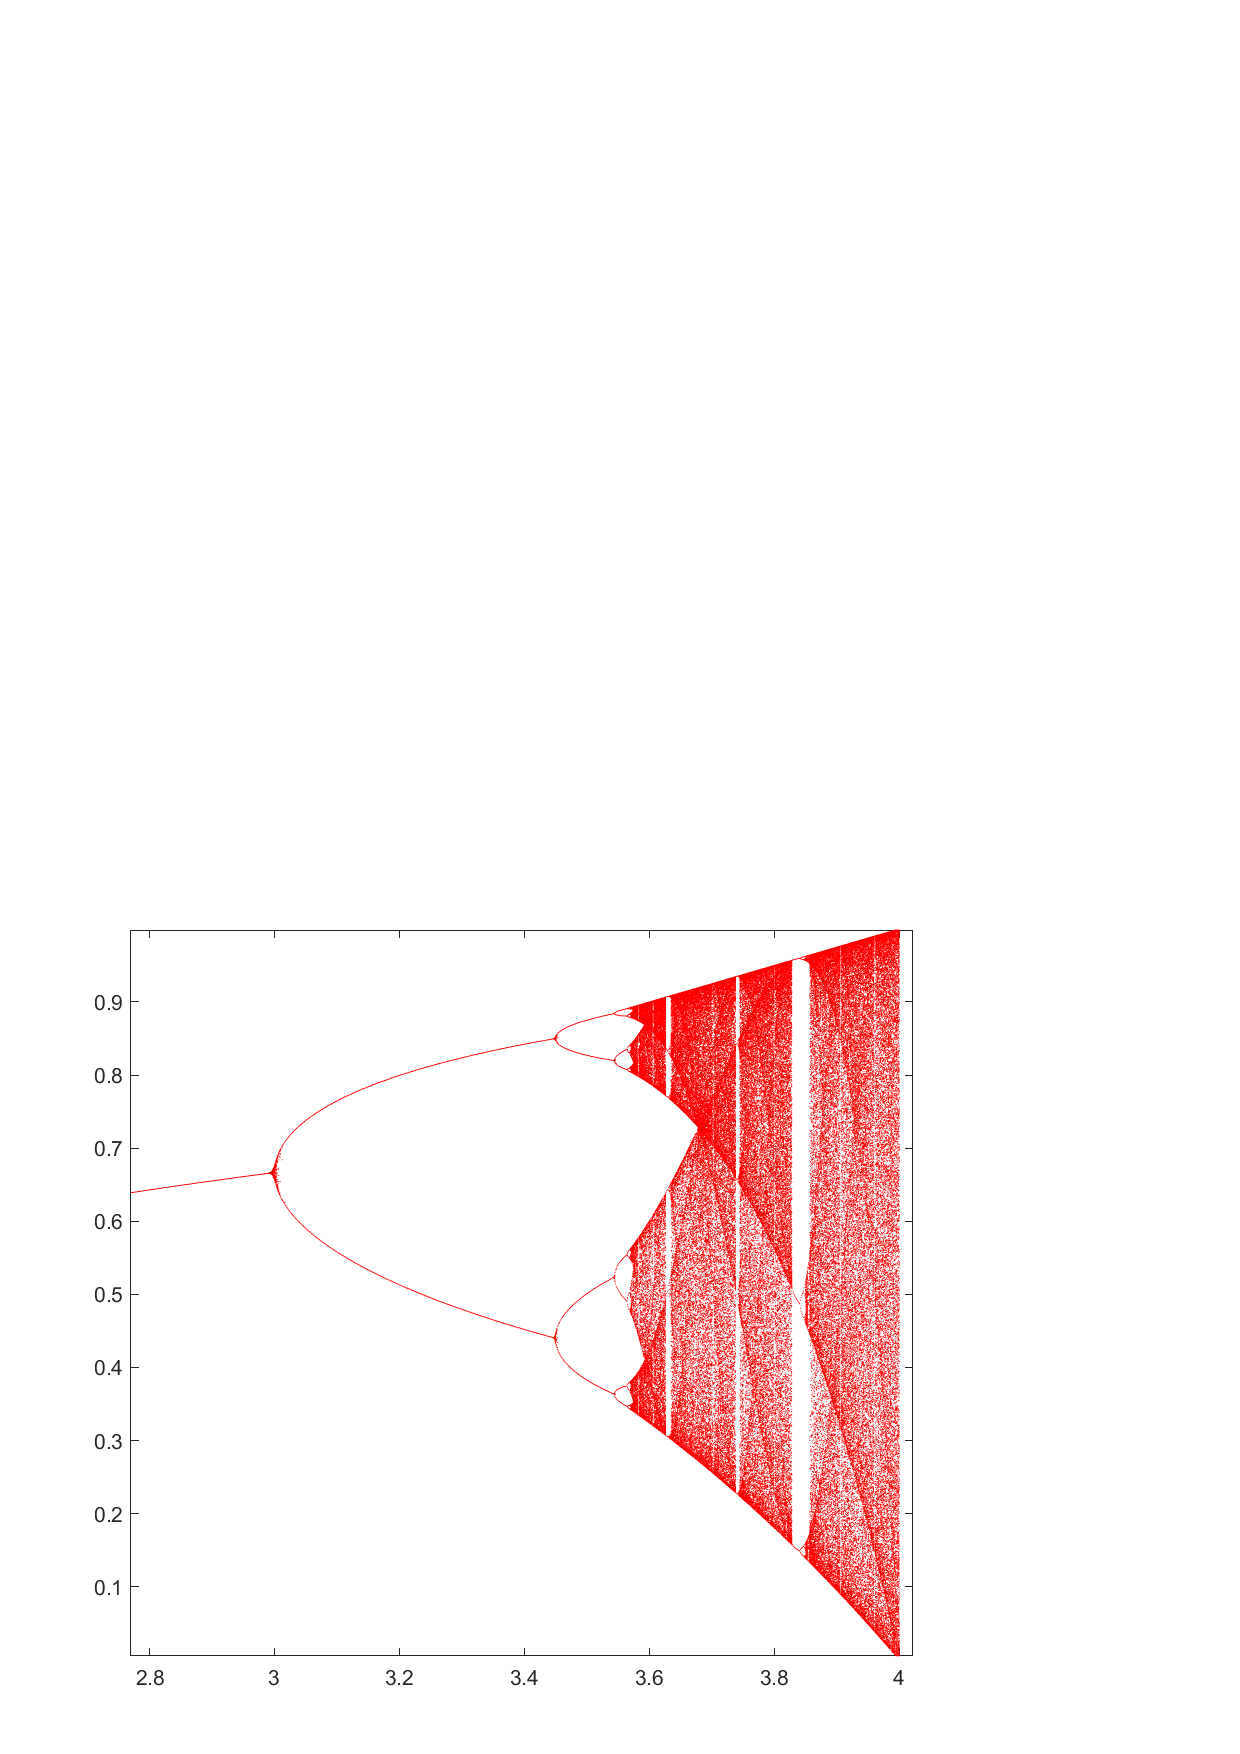
\includegraphics[scale=0.5]{logistic_1}
	\caption{Bifurcation diagram, for $2.8 \leq a \leq 4$.}
	\label{fig:logistic_1}
\end{figure}
\begin{figure}[!htb]
	\centering
	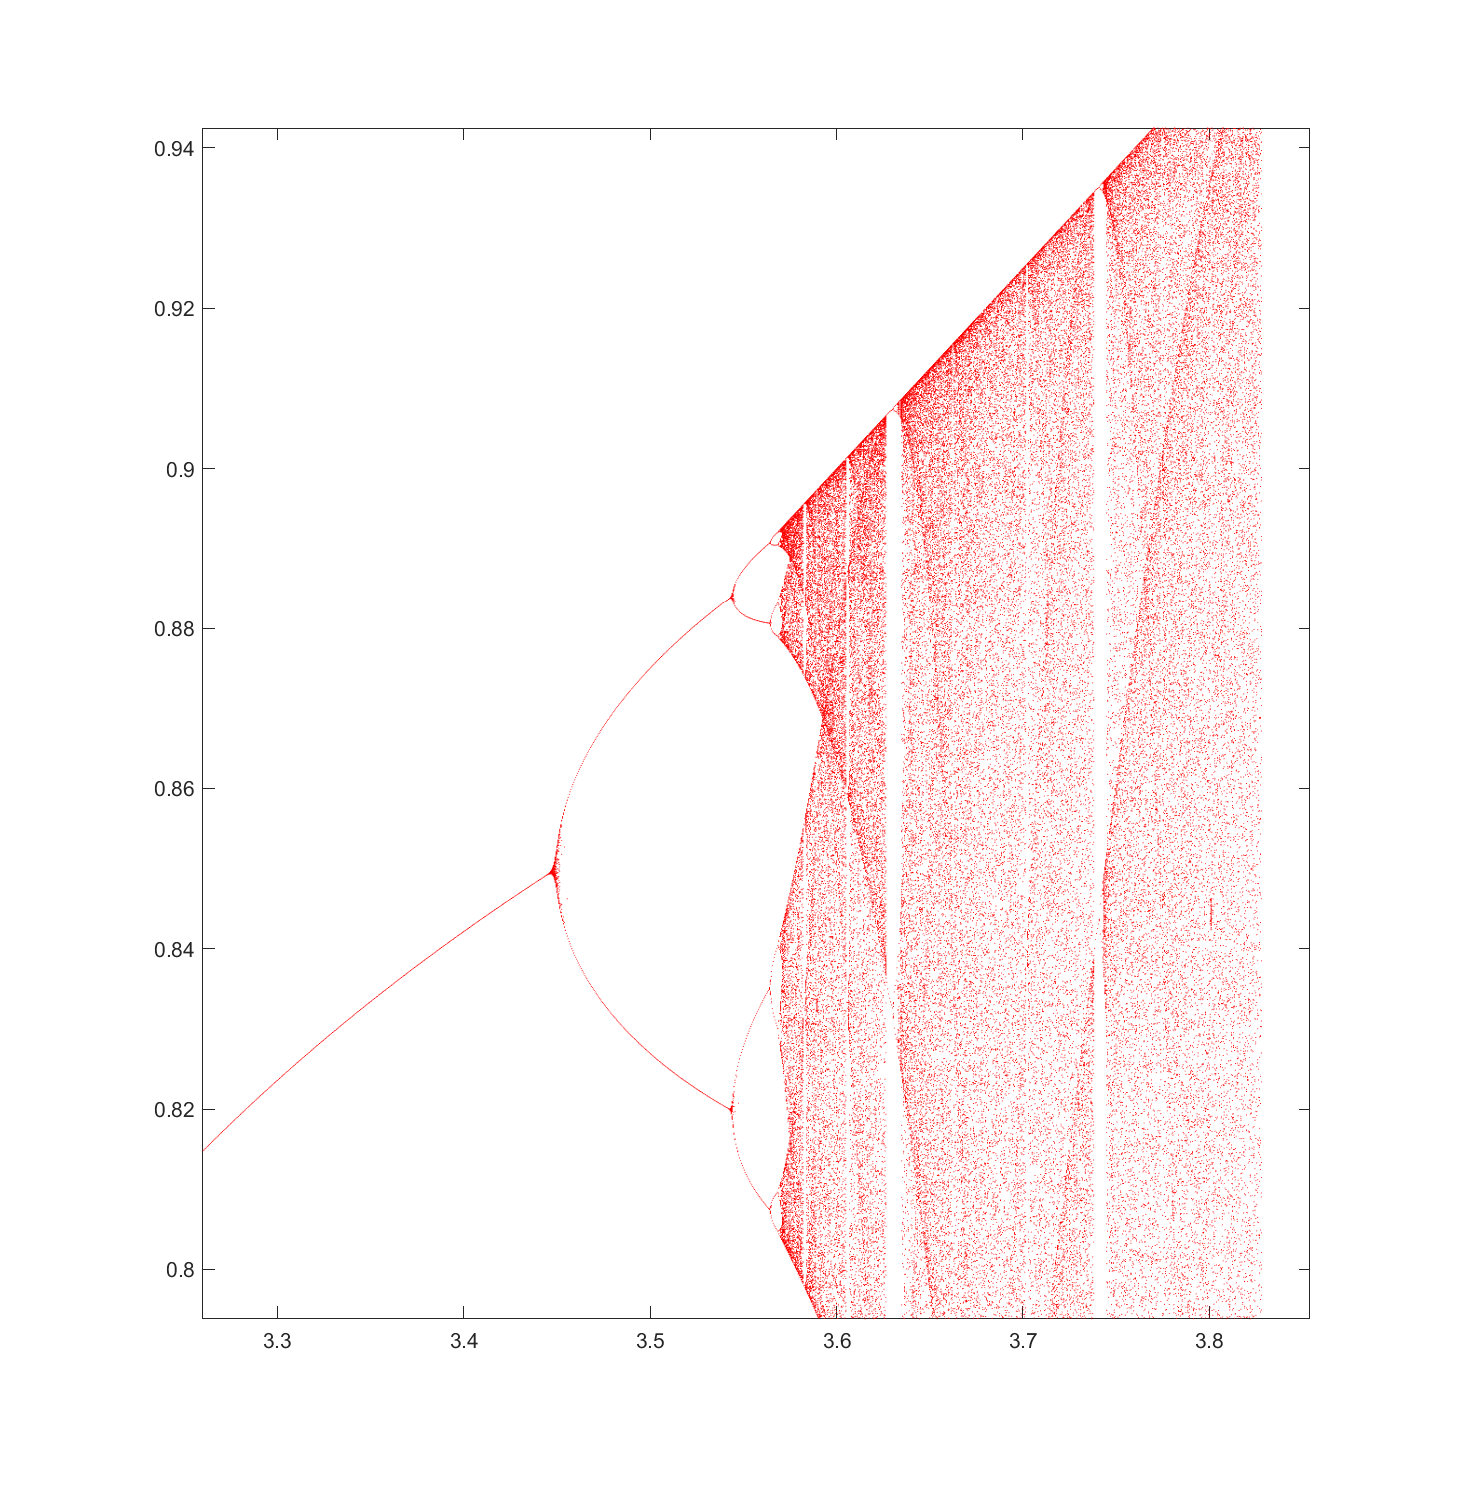
\includegraphics[scale=0.35]{logistic_3}
	\caption{Bifurcation diagram, for $3.3 \leq a \leq 3.8$}
	\label{fig:logistic_3}
\end{figure}
\begin{figure}[!htb]
	\centering
	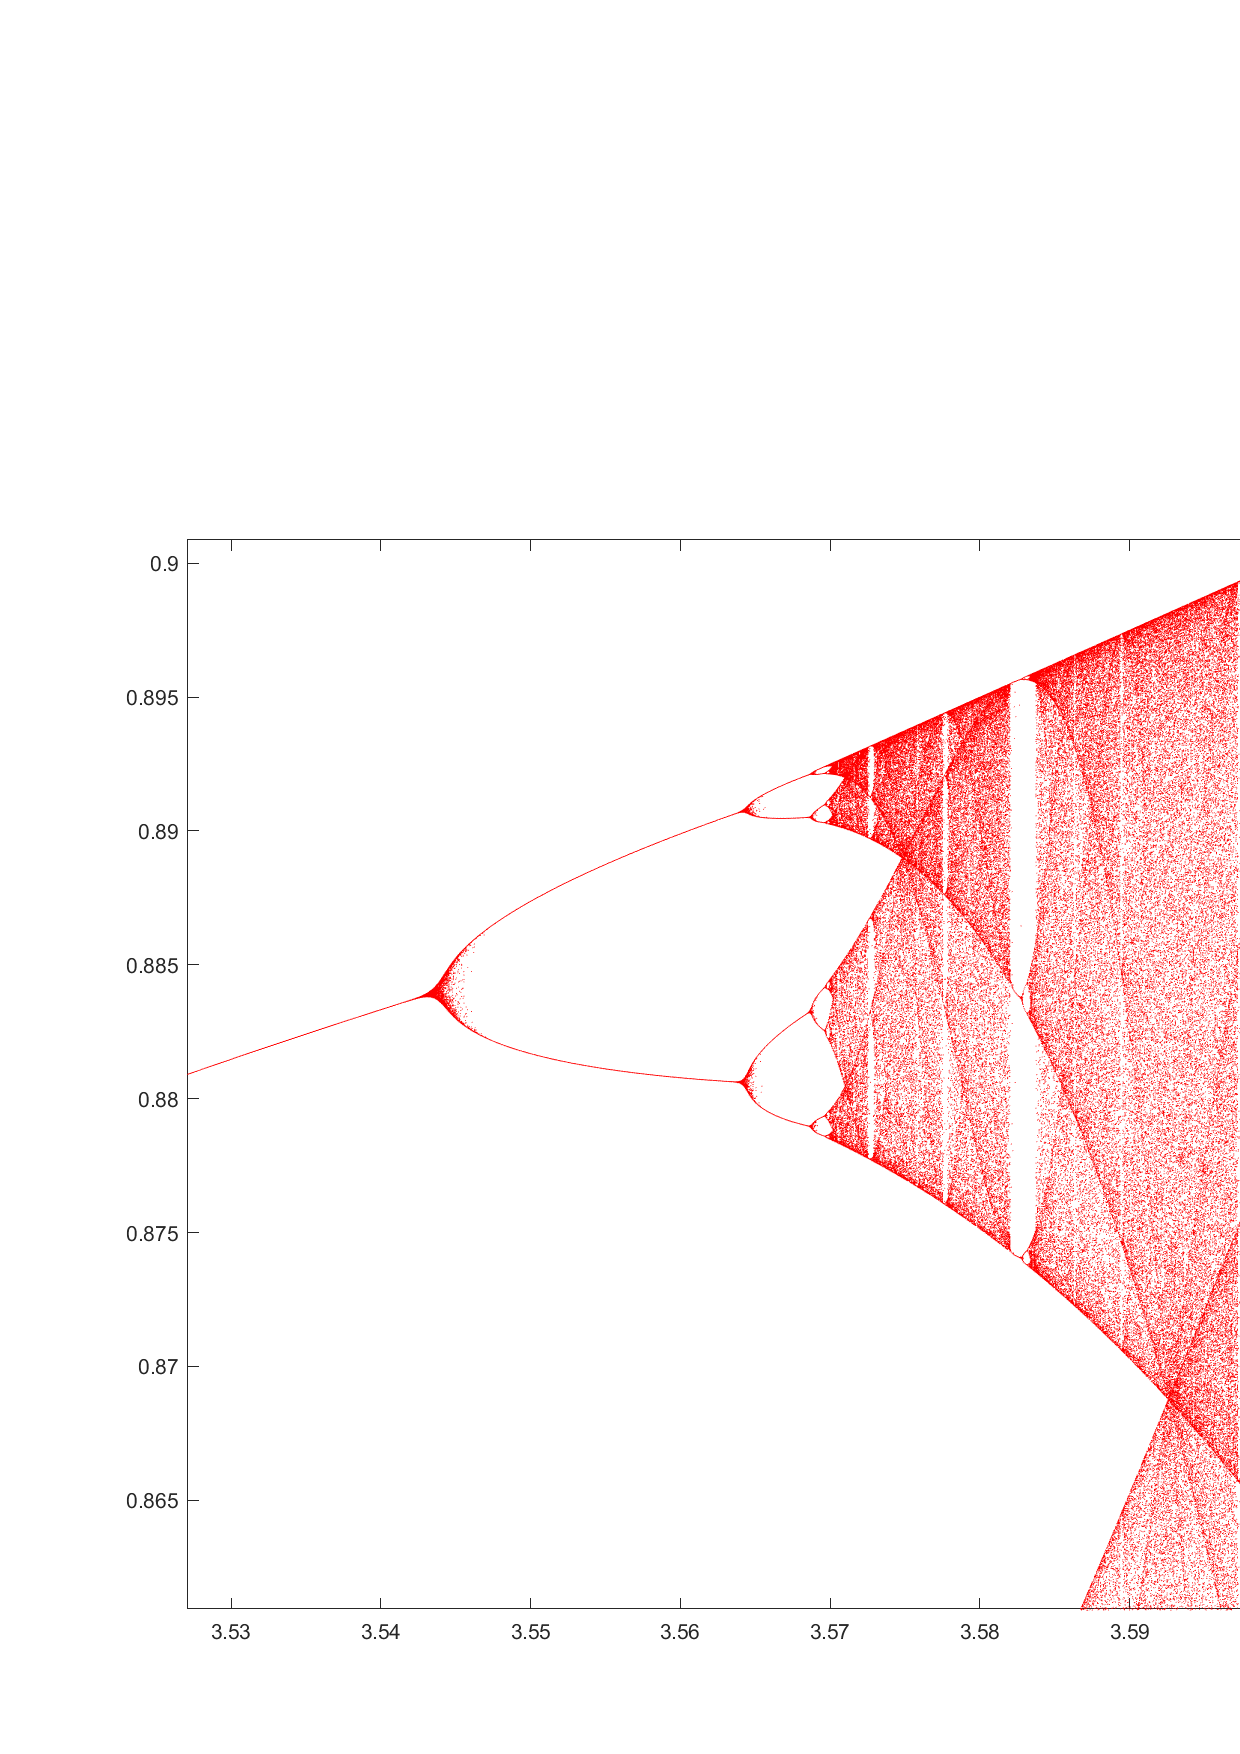
\includegraphics[scale=0.35]{logistic_4_top_branch_1}
	\caption{Bifurcation diagram, for $3.53 \leq a \leq 3.6$.}
	\label{fig:logistic_4}
\end{figure}
\begin{figure}[!htb]
	\centering
	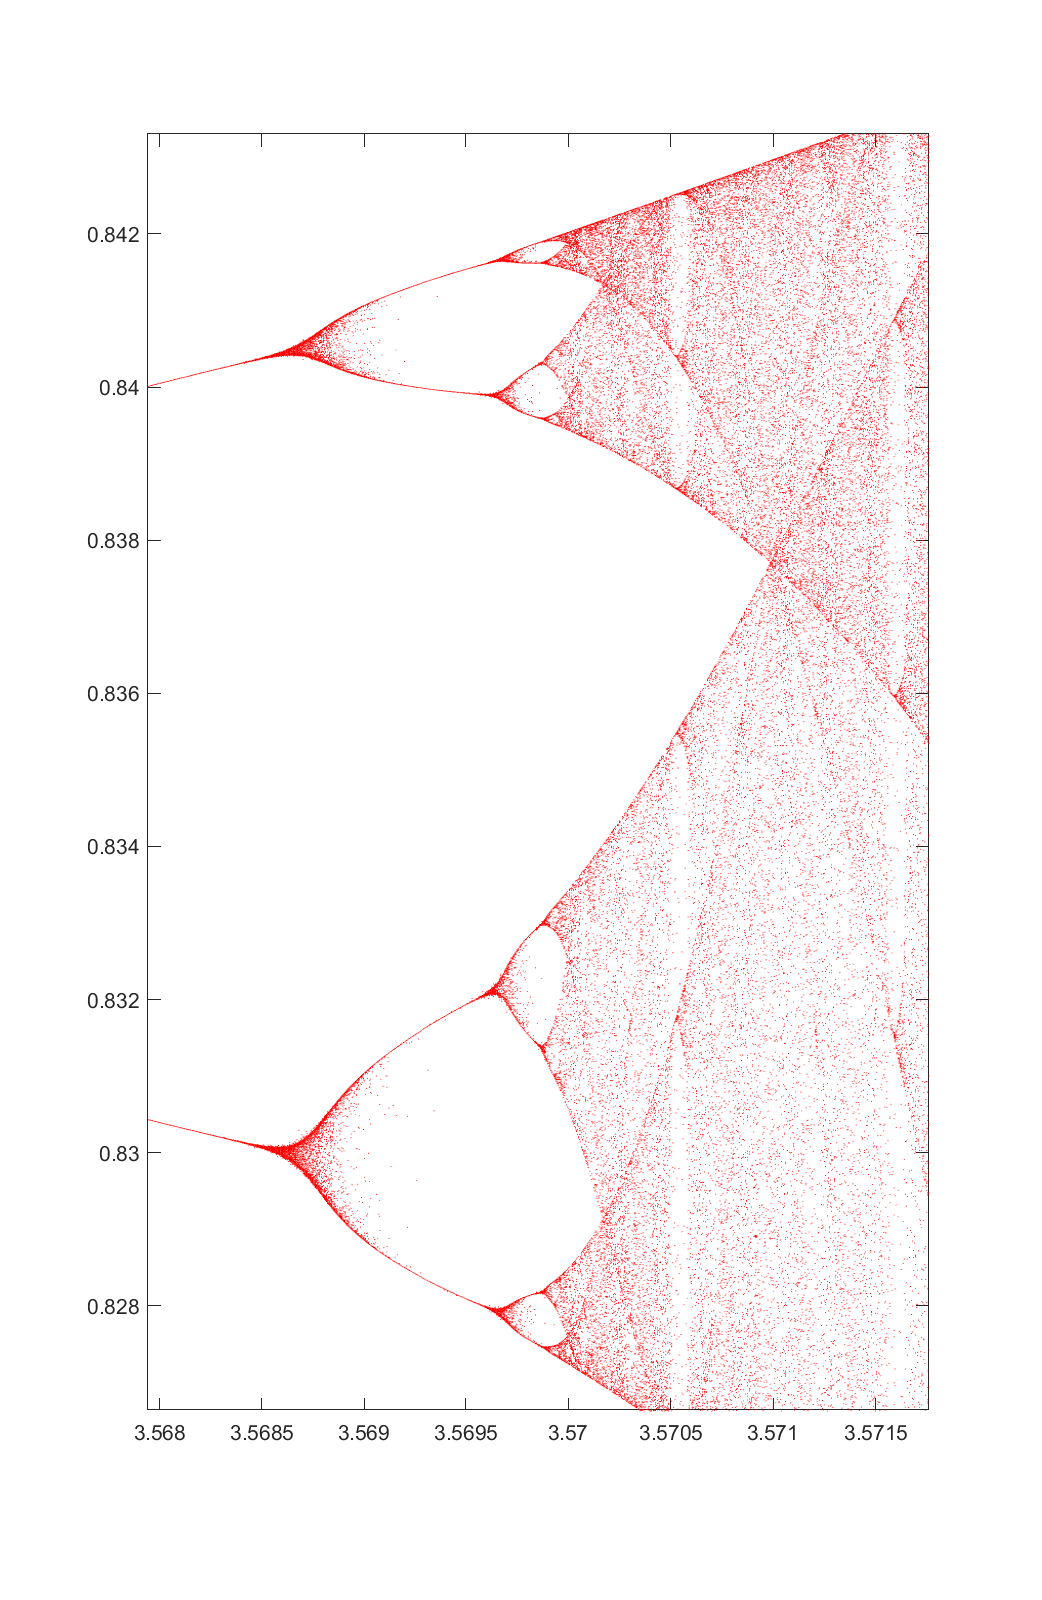
\includegraphics[scale=0.4]{logistic_5_more_branches}
	\caption{Bifurcation diagram, for $3.568 \leq a \leq 3.5715$.}
	\label{fig:logistic_5}
\end{figure}


Since the distance $|a_{n} - a_{n-1}|$ becomes vanishingly small as $n\to \infty$, resolving these $a_{n}$'s becomes increasingly difficult and requires more and more precise simulations. Fortunately, the period-doubling cascade that is related to the initial doubling (which we will call ``cascade of the first order'')  stops appearing at $a_\infty\approx 3.57$ (see Figure \ref{fig:logistic_5}). Beyond this point, the system is almost always chaotic except for certain regions which appear as blank, vertical stripes in the bifurcation diagram. Within these stripes, however, there are more period-doubling cascades of higher order beyond $a_\infty$ that are not related to the first-order cascade. We will explore these in the next section, where more precise computer simulations are shown.




\subsection{More Period-Doubling}


Figure \ref{fig:odd_period_1} shows various final states of the system for $3.558 < a < 3.95$. Recall from the preceding section that the period-doubling cascade of the first order stops at $a_\infty \approx 3.57$. However, there are clearly higher-order period-doubling cascades for $a>a_\infty$. At $a \approx 3.82$, for instance, we see the onset of a different period-doubling cascade. Here, the final states of the system can take on 3 values. For $ 3.842 < a < 3.847$, we see that the 3 values double to 6, then 12, 24, and so on. We are now in yet another period-doubling cascade. 



\begin{figure}[!htb]
	\centering
	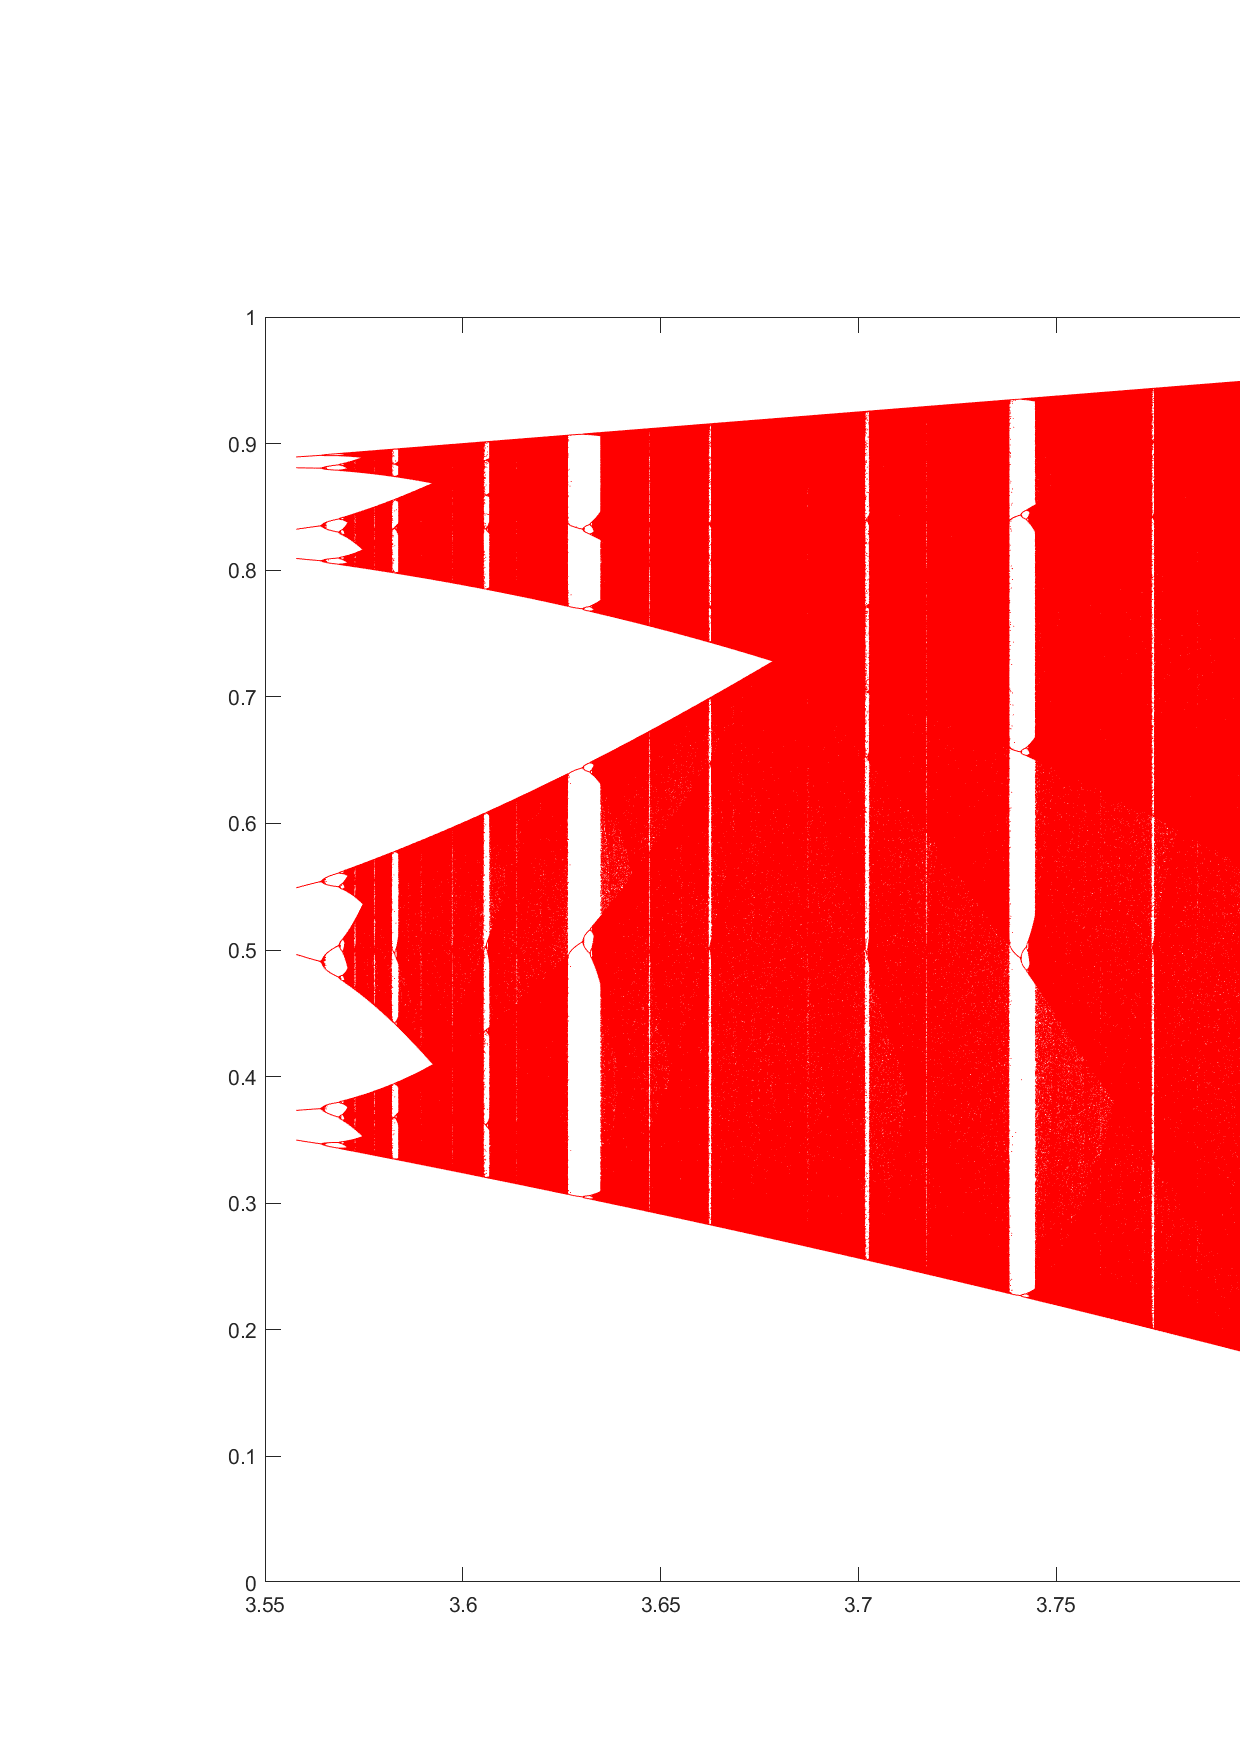
\includegraphics[scale=0.26]{odd_period_1}
	\caption{$3.558 < a < 3.95$}
	\label{fig:odd_period_1}
\end{figure}


The keen reader might now realize that at every ``blank stripe'' on the bifurcation diagram there begins a new period-doubling cascade. For example, from Figure \ref{fig:odd_period_1} we see that the system can eventually take on 5, 6, 10  values, each resulting in their own cascade! 

\begin{figure}[!htb]
	\centering
	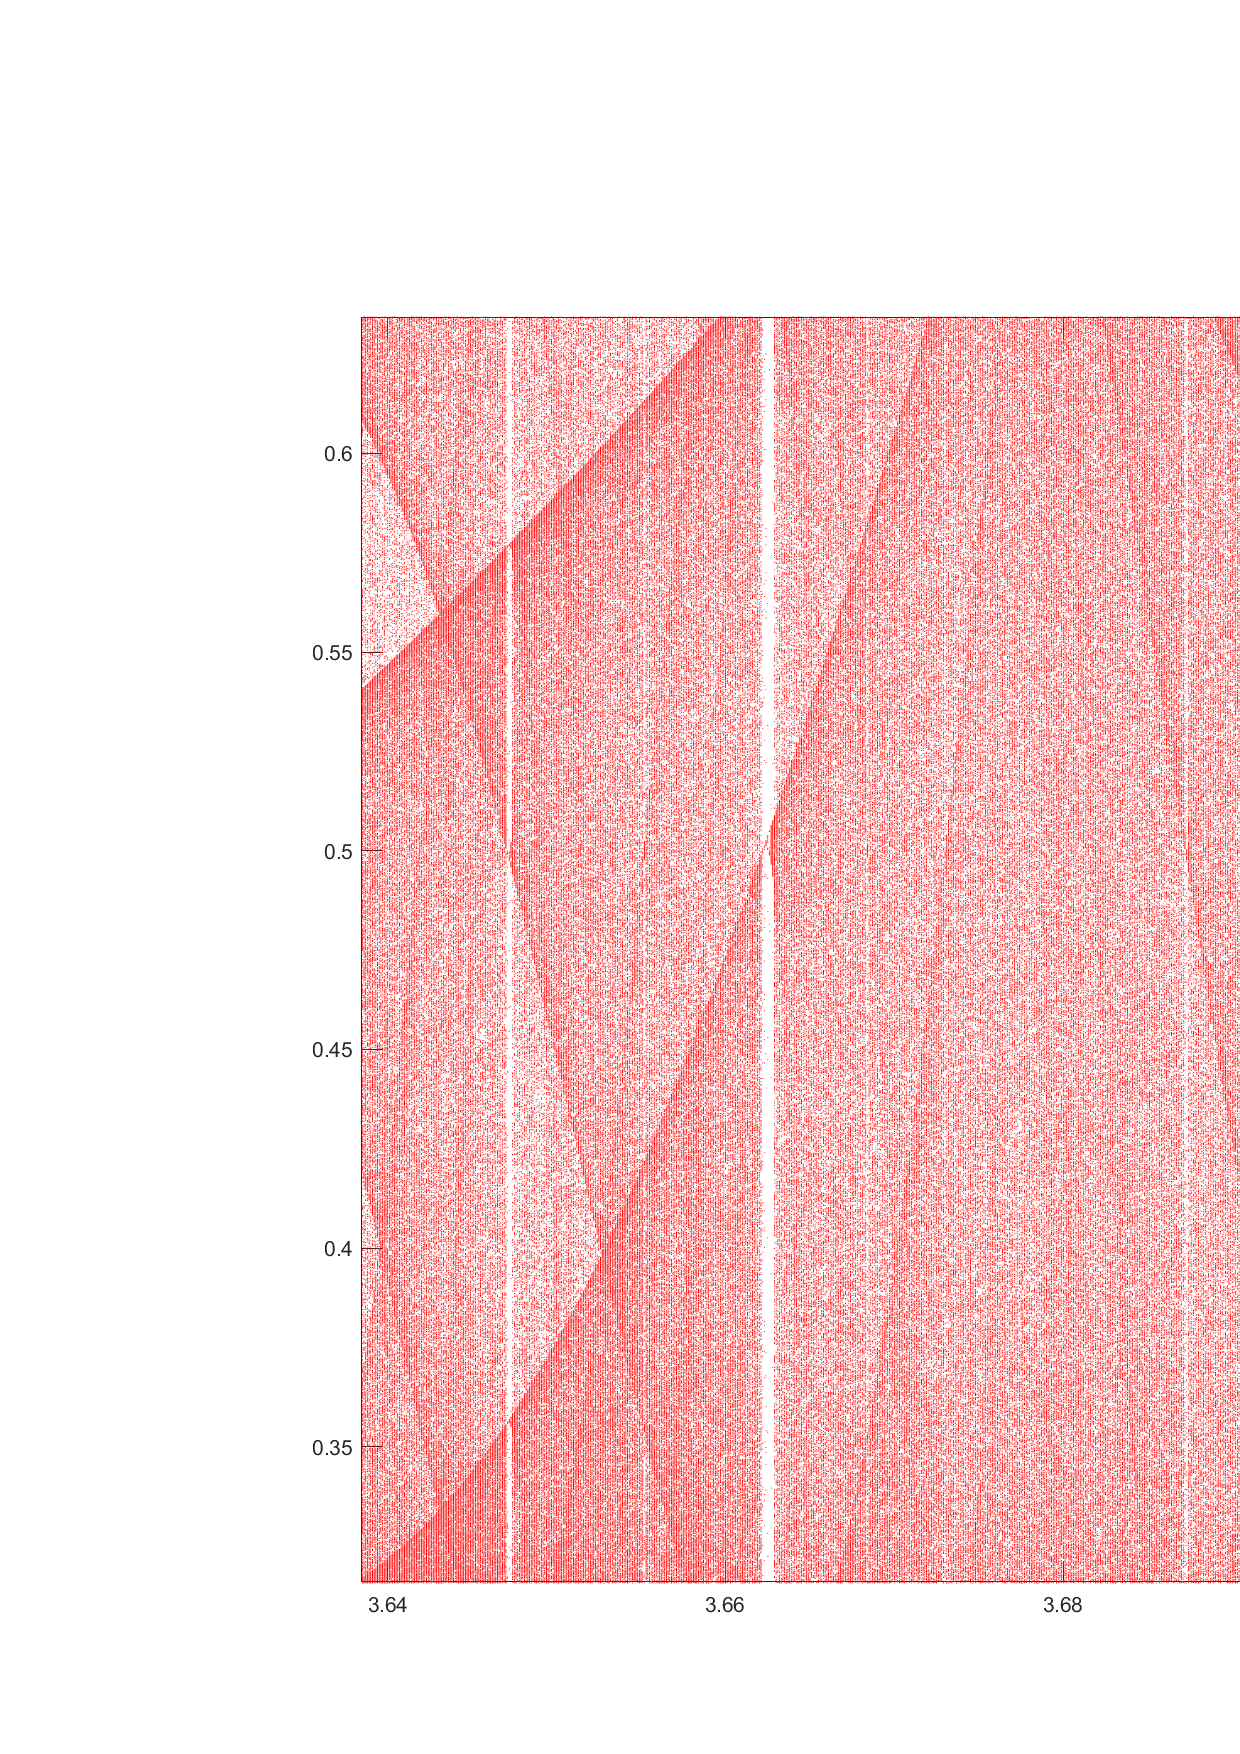
\includegraphics[scale=0.18]{odd_period_2}
	\caption{$3.64 < a < 3.77$}
	\label{fig:odd_period_2}
\end{figure}


Notice that even these cascades are only those which we can resolve from the bifurcation diagram above. Just as before, by zooming into each bifurcation and studying it in better detail, one will be able to resolve even more onsets of period-doubling cascades (see Figure \ref{fig:odd_period_2}, for example).

There is still much more to the story, and the already enormous complexity here makes it easy to forget that we started with a very simple mathematical rule! 




\subsection{The First Feigenbaum constant}

Let us press on and return to the first-order period-doubling cascade to explore the Feigenbaum constants. In the subsection about the first-order period-doubling, we have seen that the distance $|a_{n+1} - a_n|$ becomes vanishingly small as $n\to \infty$ and $a_n \to a_\infty \approx 3.57$. The excited reader might wonder at what rate this distance is decreasing. The Feigenbaum constants address this question. 


There are two Feigenbaum constants $\delta$ and $\alpha$. In this paper, we will only focus on $\delta$, which is defined as 
\begin{equation}
\delta = \lim_{n\to \infty} \frac{a_{n+1} -a_n}{a_{n+2} - a_{n+1}} \nonumber.
\end{equation}
Just as the inverse golden ratio $1/\varphi$ is defined as the limiting ratio of the difference between two consecutive terms in the Fibonacci sequence to the next, $\delta$ is the limiting ratio of each bifurcation interval to the next between every period doubling. There is no known closed form for $\delta$. However, clever computational methods have been able to give us at least a thousand digits of $\delta$, which is approximately $4.669$ \cite{feigenbaum_delta}. There are two amazing facts here. First, it is that this ratio converges to a single number rather than behaving ``chaotically.'' Second, it is that $\delta$ arises \textit{universally} not only in each of the $n$th-order period-doubling cascade for the logistic map but also in systems approaching chaos via period-doubling \cite{feigenbaum}. 

For brevity, we will not discuss the second Feigenbaum constant, $\alpha$, here. However, the reader is highly encouraged to explore and compute it!



\subsection{Connection to the Mandelbrot Set}


Just as an aside, the mathematically inclined reader will find that one can easily transform the logistic map 
\begin{equation}
x_{n+1} = ax_n(1-x_n)\nonumber
\end{equation}
into the fractal map corresponding to the Mandelbrot set
\begin{equation}
z_{n+1} = c + z_n^2 \nonumber
\end{equation}
by a simple change of parameters. To see the deeper correspondence between the logistic map and the Mandelbrot set, we first notice that the Mandelbrot set intersects the real axis on the interval $[-2,-1/4]$. From here, we can transform the logistic map such that $a$ now ranges from $-2$ to $-1/4$. Plotting the full bifurcation diagram and the Mandelbrot set on the same figure illustrates this amazing correspondence: for every new bifurcation on the diagram there is a new petal of the Mandelbrot set (see Figure \ref{fig:mandelbrot}). Mathematically, this should come as no surprise because we have transformed the original logistic map to match the form of the fractal map. However, the graphical correspondence is still very satisfying to see.


\begin{figure}[!htb]
	\centering
	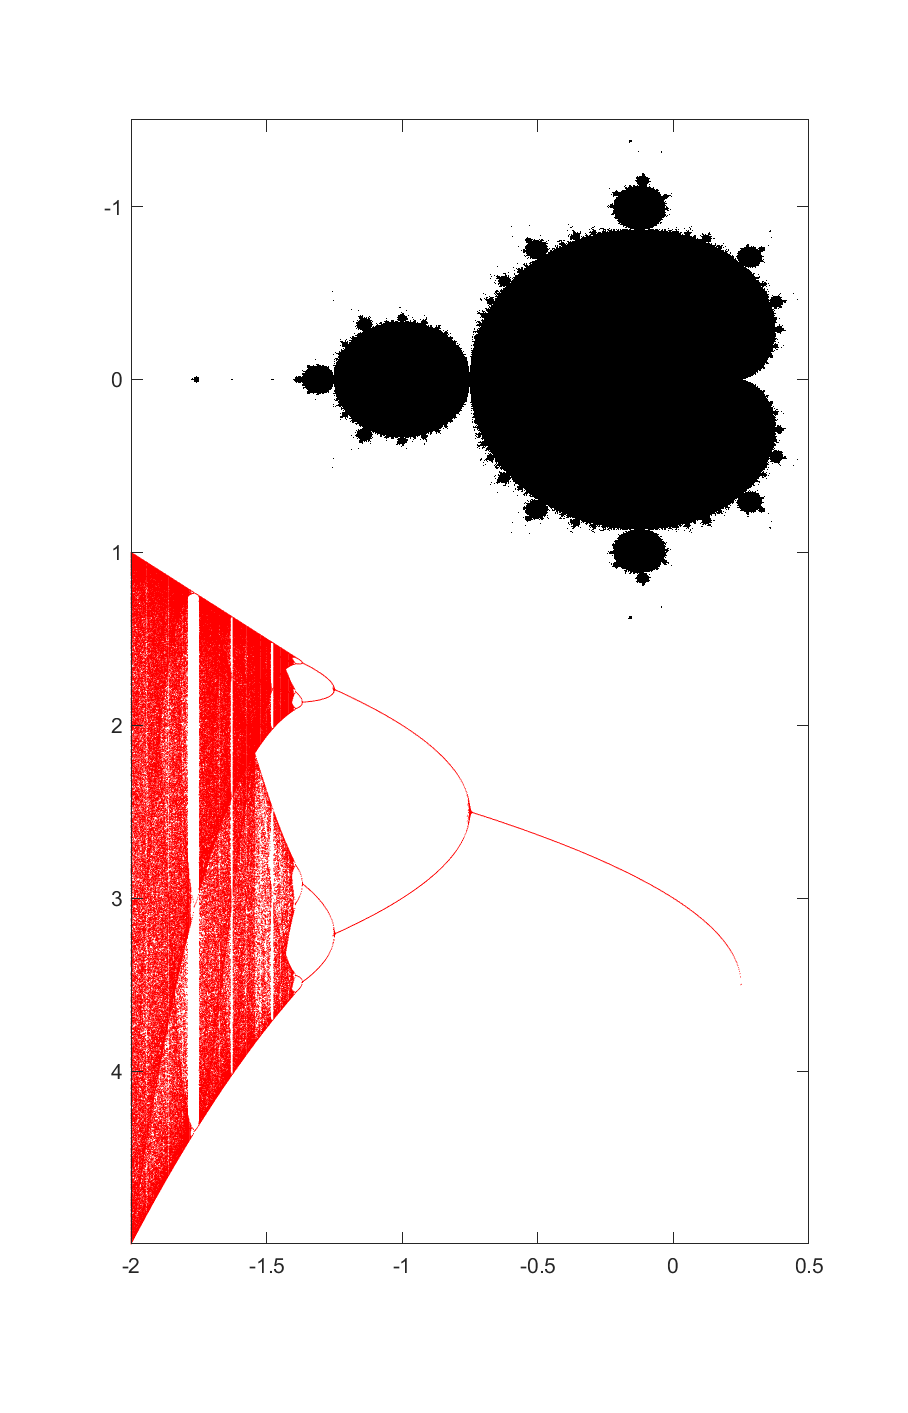
\includegraphics[scale=0.45]{mandelbrot_1}
	\caption{Bifurcation diagram and the Mandelbrot set}
	\label{fig:mandelbrot}
\end{figure}



\section{Summary}


So, just how complicated is the complicated dynamics arising from the simple logistic map? This paper attempts to address this question by investigating in detail the bifurcation diagram associated with this map. We first observe the first-order period-doubling cascade. Next, we find that in certain ``regions of stability'' more period-doubling cascades emerge. While these cascades can appear at different locations in the parameter space, they are self-similar and similar to each other, sharing the mysterious yet characteristic Feigenbaum constants $\delta$ and $\alpha$. Finally, because of its mathematical form, the logistic map can be transformed into a fractal map which generates the Mandelbrot set. As a result, the Mandelbrot set corresponds beautifully with the bifurcation diagram. 

Since this paper is only expository in nature, it has left out many other fascinating aspects of the chaos that emerge from the logistic map. For instance, mathematicians are still unsure whether the Feigenbaum constants $\delta$ and $\alpha$ are transcendental. There are also numerous other mathematical results related to the period-doubling property of the logistic map. This paper has only barely scratched the surface of what is evidently an enormous collection of phenomena and open problems that emerge from this simple mathematical rule. 




\bibliography{paper2}


\end{document}